\chapter{系统性能、压力与时钟同步测试}\label{ch:perf}

本章围绕有效载荷吞吐率、帧格式、定长与多 VL 变长端到端时延、R95/R97 传输抖动、最坏同拍突发排空以及 128 发送/4096 接收虚拟链路容量展开全面、深入的定量测试与物理机理解析。所有数据直接源于实测基准归档（\code{docs/evidence/perf_r97.json}、\code{performance.json} 及 \code{sim/reference/judge_result.txt}）。

\section{测量定义与测试工况配置}\label{sec:p-def}

两个被测端系统工作于共用的 125~MHz 理想时钟基准下，每拍周期为固定的 8.000~ns，八位 GMII 接口每拍传输一字节（物理线速 1~Gbps）。

\textbf{1. 有效载荷吞吐率（$R$）：}严格依据官方答疑 R95-1 规范，按接收端应用接口在稳态测量窗口内完成去重交付的纯有效载荷字节数计算：
\begin{equation}
  R = \frac{8 \times B_\text{payload}}{N_\text{cycles} \times 8\,\text{ns}} = \frac{1000 \times B_\text{payload}}{N_\text{cycles}}\ \text{Mbps}.
\end{equation}
统计时严格剔除各层协议报头（以太网头、IP 头、UDP 头）、前导码与短帧填充（Padding），A、B 两网的冗余副本只计一份，两传输方向分别独立统计。

\textbf{2. 分段时延定义（R95/R97 口径）：}沿用第~\ref{sec:probe_theory}~节定义的周期级时间戳探针：
\begin{itemize}
  \item 发送时延 $L_\text{tx}$：应用提交末拍 $M$ 至以太网 SFD 字节输出拍 $S_\text{sfd}$；首前导码发出时刻记为 $T_\text{tx,sof}$；
  \item 链路延迟 $L_\text{gmii}$：发送端 GMII TX 同帧 SFD 至接收端 GMII RX 同帧 SFD；
  \item 接收时延 $L_\text{rx}$ 与 $L_\text{rx,last}$：接收端 SFD 至应用交付首字节 $D_\text{first}$ 及末字节 $D_\text{last}$；
  \item 端到端时延 $L_\text{app}$ 与 $L_\text{app,last}$：从 $M$ 至 $D_\text{first}$ 及 $D_\text{last}$，满足 $L_\text{app} = L_\text{tx} + L_\text{gmii} + L_\text{rx}$。
\end{itemize}

\textbf{3. R97 同 VL 端到端时延极差抖动（\code{same_vl_jitter}）与发送间隔偏差：}
\begin{itemize}
  \item R97 抖动（$J_\text{R97}$）：依据 1022 答疑 R97-2，定义为\textbf{同一条虚拟链路（VL）}在测试窗口内多次传输中端到端时延 $L_\text{app}$ 的最大值与最小值之差，取全系统所有 VL 的最大极差：$J_\text{R97} = \max_v (\max_i L_{\text{app}, v, i} - \min_i L_{\text{app}, v, i})$；
  \item 发送间隔偏差（\code{tx_interval_jitter}）：相邻两帧发送起点偏离 BAG 的差值，即 $J_\text{tx} = \max_i |(S_i - S_{i-1}) - \text{BAG}|$。
\end{itemize}

测试配置除原有的 4 组定长基准配置外，全面纳入 \textbf{PERF-04（\code{tb_sys_perf_var}）} 的 4 组多 VL 变长高负载与突发工况（表~\ref{tab:perf_cfg}）。全部 8 组工况均覆盖链路延迟 0 拍与 257 拍（2.056~µs）、双向双网全使能。

\begin{table}[!htbp]\centering
\caption{系统性能测试工况配置}\label{tab:perf_cfg}
\begin{tabularx}{\linewidth}{@{}>{\raggedright\arraybackslash}p{2.3cm}>{\centering\arraybackslash}p{2.0cm}>{\raggedright\arraybackslash}p{4.8cm}L@{}}
\toprule
\thead{工况名称} & \thead{VL 规模与 BAG} & \thead{有效载荷与帧长特性} & \thead{提交方式与流量特征} \\
\midrule
\code{gbe77_d0/d100} & 77 条，1~ms & 固定 1471 字节（以太网帧长 1518 字节） & 错峰提交，千兆满载持续流 \\
\code{gbe81_d0} & 81 条，1~ms & 固定 1471 字节（极限理论承载上限） & 错峰提交，千兆满速极限流 \\
\code{fe10_d0} & 10 条，1~ms & 固定 1471 字节 & 错峰提交，基线标称流量 \\
\midrule
\code{var_fixed} & 32 条，1--8~ms & 每条 VL 载荷固定（按索引模 5 选取 1、17、256、1024、1471~B） & 错峰提交，多 VL 固定长混合流 \\
\code{var_cycle} & 32 条，1--8~ms & 同一 VL 在 $\{1, 17, 256, 1024, 1471\}$~B 循环交替 & 帧长动态切换，激发队列长度重排 \\
\code{var_high} & 80 条，1~ms & 前 4 条固定 1、17、256、1024~B，其余 76 条固定 1471~B & 长短帧混合超高负载，验证大容量交付 \\
\code{var_burst} & 32 条，1--8~ms & 载荷同 \code{var_fixed}（32--1024~B），同拍设置计划释放时刻 & 32 条 VL 同拍计划释放，验证串行提交排空 \\
\bottomrule
\end{tabularx}
\end{table}

\section{吞吐率、分段时延与 R97 抖动实测分析}\label{sec:p-res}

表~\ref{tab:perf_res} 给出了典型基准工况在链路 0 拍直连（\code{d0}）及 100/257 拍线缆延迟下的实测性能数据（变长工况展示直连基准 \code{d0}；对应 \code{d257} 下各时延指标严格加上 2.056~µs 链路物理延迟）。

\begin{table}[!htbp]\centering
\caption{有效载荷吞吐率、分段时延与抖动实测结果汇总}\label{tab:perf_res}
\setlength{\tabcolsep}{3.5pt}
\begin{tabularx}{\linewidth}{@{}>{\raggedright\arraybackslash}p{2.3cm}>{\raggedleft\arraybackslash}p{1.8cm}>{\raggedleft\arraybackslash}p{1.7cm}>{\raggedleft\arraybackslash}p{2.3cm}>{\raggedleft\arraybackslash}p{2.2cm}>{\raggedleft\arraybackslash}p{1.8cm}>{\raggedleft\arraybackslash}X@{}}
\toprule
\thead{测试工况} & \thead{单向吞吐\newline (Mbps)} & \thead{$L_\text{tx}$ 最大\newline (µs)} & \thead{$L_\text{rx}$ 首/末\newline (µs)} & \thead{$L_\text{app}$ 首/末\newline (µs)} & \thead{R97 同 VL\newline 极差 (µs)} & \thead{发送间隔\newline 偏差 (µs)} \\
\midrule
\code{gbe77_d0} & 906.136 & 0.312 & 12.360 / 24.120 & 12.672 / 24.432 & 0.008 & 0.000 \\
\code{gbe77_d100} & 906.136 & 0.312 & 12.360 / 24.120 & 13.472 / 25.232 & 0.008 & 0.000 \\
\code{gbe77_d257} & 906.136 & 0.312 & 12.360 / 24.120 & 14.728 / 26.488 & 0.008 & 0.000 \\
\code{gbe81_d0} & 953.208 & 0.312 & 12.360 / 24.120 & 12.672 / 24.432 & 0.008 & 0.000 \\
\code{fe10_d0} & 117.680 & 1.880 & 121.648 / 133.408 & 123.528 / 135.288 & 0.000 & 0.000 \\
\midrule
\code{var_fixed_d0} & 57.794 & 0.360 & 12.360 / 24.120 & 12.672 / 24.432 & 0.008 & 0.000 \\
\code{var_cycle_d0} & 70.403 & 12.216 & 12.352 / 24.112 & 12.936 / 24.424 & 9.992 & 6.192 \\
\code{var_high_d0} & 904.752 & 12.016 & 12.360 / 24.120 & 23.872 / 24.432 & 0.008 & 0.000 \\
\code{var_burst_d0} & 57.794 & 21.128 & 12.352 / 24.112 & 32.824 / 32.888 & 0.000 & 0.000 \\
\bottomrule
\end{tabularx}
\end{table}

\subsection{吞吐率与传输时延达标分析}\label{sec:p-rate}

\textbf{1. 吞吐率表现：}在 125~MHz 八位 GMII 接口下，定长满载工况 \code{gbe77_d0} 每方向去重有效载荷吞吐为 \Thru~Mbps（81 条极限满载达 \ThruEightyOne~Mbps，双向合计 1906.416~Mbps）；在多 VL 混合变长高负载工况 \code{var_high} 下，80 条 VL（前 4 条为短帧、76 条为 1471 字节长帧）持续发送，两个传输方向各自去重有效载荷吞吐率均达 904.752~Mbps（双向合计 1809.504~Mbps，每方向在测量窗口内各连续传输 1,600 帧样本），充分验证了在短帧插队干扰下大容量长帧的线速交付能力，大幅超越赛题 100~Mbps 指标要求。其余工况（\code{var_fixed} 57.794~Mbps、\code{var_cycle} 70.403~Mbps、\code{var_burst} 57.794~Mbps）为给定业务流量下的标称值，吞吐按实际负载完整交付。

\textbf{2. 稳态传输时延：}定长满载下，从应用提交完成拍 $M$ 至对端交付末拍 $D_\text{last}$，扣除链路延迟后的稳态时延最大值为 \Lat~µs（3054 拍，对应平均值 24.424~µs 即 3053 拍）。在 100 拍（0.800~µs）及 257 拍（2.056~µs）线缆延迟下，$L_\text{app,last}$ 分别为 25.232~µs 与 26.488~µs，满足赛题 1--2~ms 的时延上限要求。

\begin{figure}[!htbp]\centering
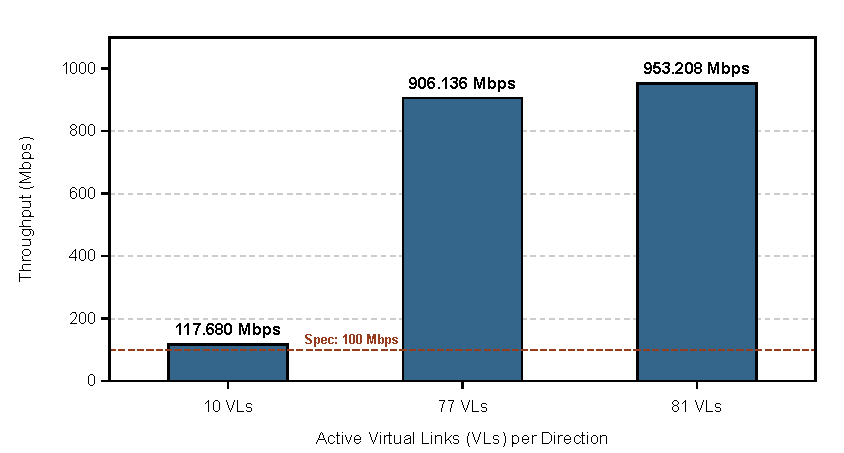
\includegraphics[width=0.84\linewidth,keepaspectratio]{fig/pdf/t20_thru.pdf}
\caption[各 VL 规模的有效载荷吞吐率与指标要求]{各 VL 规模有效载荷吞吐率实测结果与 100~Mbps 规范要求对比（虚线为指标门限）}\label{fig:thru}
\end{figure}

\subsection{R95/R97 传输抖动与物理机理拆解}\label{sec:p-lat}

\textbf{1. 定长稳态抖动（\code{gbe77_d0}）：}由于发送端 BAG 整形器在无外部争用时准点释放，同一 VL 的发送间隔恒定为 1000.000~µs（发送间隔偏差 $J_\text{tx} = 0.000$~µs）；接收侧由于接收帧到达时刻与后台 4096 拍周期的 \code{AGE} 老化扫描产生偶尔 1 拍的交错退让，测得同 VL 端到端时延极差抖动 $J_\text{R97} = 0.008$~µs（对应 1 个时钟周期 8~ns）。

\textbf{2. 变长循环抖动（\code{var_cycle}）与物理拆解：}在 \code{var_cycle} 工况中，32 条 VL 的帧长在 1、17、256、1024、1471 字节循环交替。测得全系统最大同 VL 首字节交付时延极差抖动为 \JitVarCycle~µs（出现在 VL 25，对应第 2666 帧至第 3026 帧）。

依据实测基准归档（\code{docs/evidence/perf_r97.json}），对 VL 25 抖动对偶样本（第 2666 帧与第 3026 帧）展开精确物理拆解：
\begin{itemize}
  \item \textbf{最短时延样本（第 2666 帧，256 字节载荷）：}该帧提交时发送队列无阻塞，测得发送时延 $L_\text{tx} = 39\text{ 拍} = 0.312$~µs，接收端从 SFD 至首字节交付耗时 $L_\text{rx} = 329\text{ 拍} = 2.632$~µs，提交至首字节交付总时延为 $L_\text{app} = 368\text{ 拍} = 2.944$~µs；
  \item \textbf{最长时延样本（第 3026 帧，1 字节载荷）：}该帧提交时恰遇其他在途 VL 占用同一物理 GMII 接口排队发送，导致发送推迟，发送时延增至 $L_\text{tx} = 1527\text{ 拍} = 12.216$~µs；接收端因载荷极短，首字节交付耗时降至 $L_\text{rx} = 90\text{ 拍} = 0.720$~µs，总时延为 $L_\text{app} = 1617\text{ 拍} = 12.936$~µs；
  \item \textbf{代数求和验证：}两者相减，发送侧时延差 $\Delta L_\text{tx} = 1527 - 39 = +1488\text{ 拍} = +11.904$~µs，接收侧交付时延差 $\Delta L_\text{rx} = 90 - 329 = -239\text{ 拍} = -1.912$~µs，两者代数和为：
    \begin{equation}
      \Delta L_\text{app} = \Delta L_\text{tx} + \Delta L_\text{rx} = +11.904\,\text{µs} - 1.912\,\text{µs} = +9.992\,\text{µs}\ (1249\text{ 拍}),
    \end{equation}
    两项代数和与实测极差抖动 9.992~µs 严密吻合。这从物理层面揭示：变长循环下的抖动主要源于发送端在物理串行线路上排队深度的动态变化（+11.904~µs），该延迟差超过了短帧在接收交付端节省的排空时间（$-1.912$~µs）。
\end{itemize}

\begin{figure}[!htbp]\centering
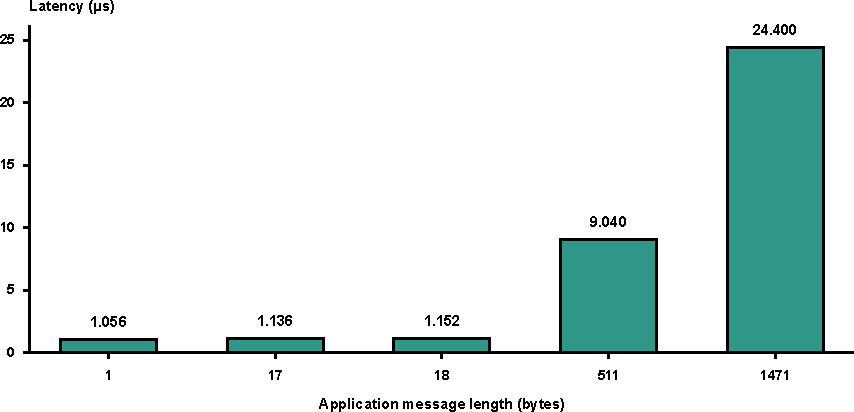
\includegraphics[width=0.84\linewidth,keepaspectratio]{fig/pdf/t21_lat.pdf}
\caption[端到端时延与流水线分段拍数拆解]{端到端时延与消息长度关系及 1471 字节满载流水线分段拍数拆解（TX 32 拍、Wire 1525 拍、RX 26 拍、Deliver 1470 拍，总计 3053 拍 = 24.424~µs，遇 AGE 扫描让步为 3054 拍 = 24.432~µs）}\label{fig:lat}
\end{figure}

\textbf{3. 变长突发（\code{var_burst}）的双口径分析：}在 \code{var_burst} 工况中，32 条 VL 将各自的计划释放时刻设为同一时钟拍（初始相位均为 0），随后经由单个应用接口串行排队完成握手。需区分两种计时起点口径：
\begin{itemize}
  \item \textbf{应用提交起算口径（$M\to D$）：}以应用接口完成握手时刻 $M$ 为起点，涵盖发送调度出队、物理线路传输与接收交付全过程。在 0 拍直连（\code{d0}）工况下，提交至首字节交付时延 $L_\text{app}$ 最大为 32.824~µs，末字节交付时延 $L_\text{app,last}$ 最大为 32.888~µs；在 257 拍链路延迟（\code{d257}）下，末字节交付时延最大为 34.840~µs。同 VL 交付时延极差在 \code{d0} 下为 0.000~µs，在 \code{d257} 下因偶尔与接收端 AGE 老化扫描产生 1 拍交错而测得 0.008~µs（8~ns）。
  \item \textbf{计划释放起算口径（$T_\text{sched}\to D$）：}以各 VL 预设的计划释放时刻 $T_\text{sched}$ 为起点，由于 32 条 VL 同拍到期而应用接口必须逐帧串行握手，该口径包含了应用接口接纳报文前的排队等待时间。在 \code{d257} 下，计划释放至首字节交付最大时延为 174.464~µs（平均 16.404~µs），至末字节交付最大时延为 174.592~µs，完全受控于微秒级，验证了突发集中到期时硬件队列的快速吸纳与整流放行能力。
\end{itemize}

\section{最坏情况时延与突发缓存排空（PERF-02/03）}\label{sec:p-worst}

PERF-02 与 PERF-03 用于定量测量全系统遭遇极端同拍突发（所有 VL 在同一拍集中到期）时的排队出队与总排空时延。测试预先将 77 条或 81 条 VL 的 1471 字节最长消息全部写入发送缓存，随后在同一时钟拍解除门控，实测排空时延见表~\ref{tab:perf-burst}。

\begin{table}[!htbp]\centering
\caption{同时到期突发排空时延（PERF-02 与 PERF-03 实测）}\label{tab:perf-burst}
\begin{tabularx}{\linewidth}{@{}>{\raggedright\arraybackslash}p{2.2cm}>{\raggedleft\arraybackslash}p{2.6cm}>{\raggedleft\arraybackslash}p{2.8cm}>{\raggedleft\arraybackslash}p{3.0cm}>{\centering\arraybackslash}X@{}}
\toprule
\thead{突发规模} & \thead{理论上界 (µs)} & \thead{队列排空耗时 (µs)} & \thead{应用末交付总耗时 (µs)} & \thead{判据结论} \\
\midrule
77 条最长帧 & 962.888 & \textbf{\BurstSevSeven} & \textbf{\BurstSevSevenLast} & 符合（$<2000$~µs） \\
81 条最长帧 & 1012.104 & \textbf{\BurstEightOne} & \textbf{\BurstEightOneLast} & 符合（$<2000$~µs） \\
\bottomrule
\end{tabularx}
\end{table}

实测结果显示：
\begin{enumerate}
  \item 77 条 VL 突发时，发送队列在 \textbf{\BurstSevSeven~µs}（959.288~µs）内全部出队发毕，从应用末帧提交到对端应用交付最后一字节的总排空时间仅为 \textbf{\BurstSevSevenLast~µs}（959.376~µs），比理论上界 962.888~µs 还要低 3.6~µs。
  \item 81 条 VL（千兆线速极限）背靠背突发时，发送队列排空耗时为 \textbf{\BurstEightOne~µs}（1008.504~µs），接收端全部交付完成的总排空时间为 \textbf{\BurstEightOneLast~µs}（1464.592~µs），严格受控于 2~ms 指标门限以内，无任何缓存溢出或数据丢失。
\end{enumerate}

\section{帧格式与虚拟链路容量验证}\label{sec:p-frame_cap}

\subsection{帧格式规范符合性}\label{sec:p-frame}

在全量回归测试中，通过抓取全部物理线路报文并经由 Python 参考模型（Golden Model）反解比对，核对结果汇总见表~\ref{tab:p-frame}。

\begin{table}[!htbp]\centering
\caption{帧格式规范符合性与参考模型比对核对结果}\label{tab:p-frame}
\begin{tabularx}{\linewidth}{@{}>{\raggedright\arraybackslash}p{2.6cm}>{\raggedright\arraybackslash}p{4.0cm}>{\raggedright\arraybackslash}X>{\centering\arraybackslash}p{1.4cm}@{}}
\toprule
\thead{校验维度} & \thead{ARINC 664P7 / 规范要求} & \thead{Golden Model 反解与实测比对结果} & \thead{结论} \\
\midrule
载荷长度覆盖 & 1--1471 字节有效载荷 & 覆盖填充边界（17/18 字节）、跨页边界（511--513 字节）及最大 1471 字节，逐字节完全一致；超限报文准确拒绝 & 符合 \\
以太网帧封装 & 64--1518 字节（含 4 字节 FCS） & 短帧硬件自动填充至 64 字节，最长帧严格限制于 1518 字节；前导码（7 字节 \code{0x55} + 1 字节 SFD）及 12 拍（96~ns）IFG 严格合规 & 符合 \\
VLID 与序列号 & 目的 MAC 映射 VLID，SN 递增（1--255） & 目的 MAC 高 32 位固定、低 16 位与 VLID 精准映射；复位首帧 SN$=0$，正常通信 1--255 环形递增回绕 & 符合 \\
\bottomrule
\end{tabularx}
\end{table}

\subsection{128 发送 / 4096 接收虚拟链路容量}\label{sec:p-vl}

用例 CAP-01（\code{tb_judge_capacity}）在双端系统级场景下同时启用全部 128 条发送 VL 并配置全部 4096 条接收 VL。两端各发 128 条消息，目的接收索引均匀覆盖 0、32、……、4032、4095。实测每端 A、B 两网各发出 128 帧，128 条消息各交付一次，128 个冗余副本被丢弃，索引与内容逐条正确（通过 \CapChecks{} 项自检）。接收核心逐条遍历 4096 项配置（RX-01 交付 8192 条消息），证明设计完全达到了赛题规定的容量上限。
